\message{ !name(frontiers.tex)}%%% Version 3.3 Generated 2016/11/10 %%%
%%% You will need to have the following packages installed: datetime, fmtcount, etoolbox, fcprefix, which are normally inlcuded in WinEdt. %%%
%%% In http://www.ctan.org/ you can find the packages and how to install them, if necessary. %%%
%%%  NB logo1.jpg is required in the path in order to correctly compile front page header %%%

\documentclass[utf8]{frontiersSCNS} % for Science, Engineering and Humanities and Social Sciences articles
%\documentclass[utf8]{frontiersHLTH} % for Health articles
%\documentclass[utf8]{frontiersFPHY} % for Physics and Applied Mathematics and Statistics articles

%\setcitestyle{square} % for Physics and Applied Mathematics and Statistics articles
\usepackage{url,hyperref,lineno,microtype,subcaption}
\usepackage[onehalfspacing]{setspace}
\usepackage{color, soul}
\usepackage{amsmath}
\usepackage{booktabs}
\usepackage{multirow}

\linenumbers
\newcommand{\FR}[1]{{\small \textcolor{red}{\hl{FR: #1}}}}

% Leave a blank line between paragraphs instead of using \\


\def\keyFont{\fontsize{8}{11}\helveticabold }
\def\firstAuthorLast{Sample {et~al.}} %use et al only if is more than 1 author
\def\Authors{First Author\,$^{1,*}$, Co-Author\,$^{2}$ and Co-Author\,$^{1,2}$}
% Affiliations should be keyed to the author's name with superscript numbers and be listed as follows: Laboratory, Institute, Department, Organization, City, State abbreviation (USA, Canada, Australia), and Country (without detailed address information such as city zip codes or street names).
% If one of the authors has a change of address, list the new address below the correspondence details using a superscript symbol and use the same symbol to indicate the author in the author list.
\def\Address{$^{1}$Laboratory X, Institute X, Department X, Organization X, City X , State XX (only USA, Canada and Australia), Country X \\
$^{2}$Laboratory X, Institute X, Department X, Organization X, City X , State XX (only USA, Canada and Australia), Country X  }
% The Corresponding Author should be marked with an asterisk
% Provide the exact contact address (this time including street name and city zip code) and email of the corresponding author
\def\corrAuthor{Corresponding Author} 

\def\corrEmail{email@uni.edu}




\begin{document}

\message{ !name(frontiers.tex) !offset(241) }
\subsection{MEG vs. audio features}

Only $0.0163$\%, $0.0116$\% and $0.132$\% of the $156 \times 4681$ correlations using the /{\em pah}/, /{\em pah tah kah}/ and verb-generation data respectively are significant (after consideration of our defined thresholds). This suggests little redundancy between the MEG and audio features analyzed and supports the consideration of a combined prediction model and a much more complex connection between phenomena. Of these significant correlations, three audio features stand out as more strongly correlated to MEG data. These features correspond to sequential FFT bins that represent the frequency range 340-400 Hz. In therms of strongly correlated MEG features: the autocorrelation measure (eq. \ref{eq1}) is the most intensely correlated MEG feature across and is so across three independent components common to all three experiments.

\begin{figure}[t]
  \centering
  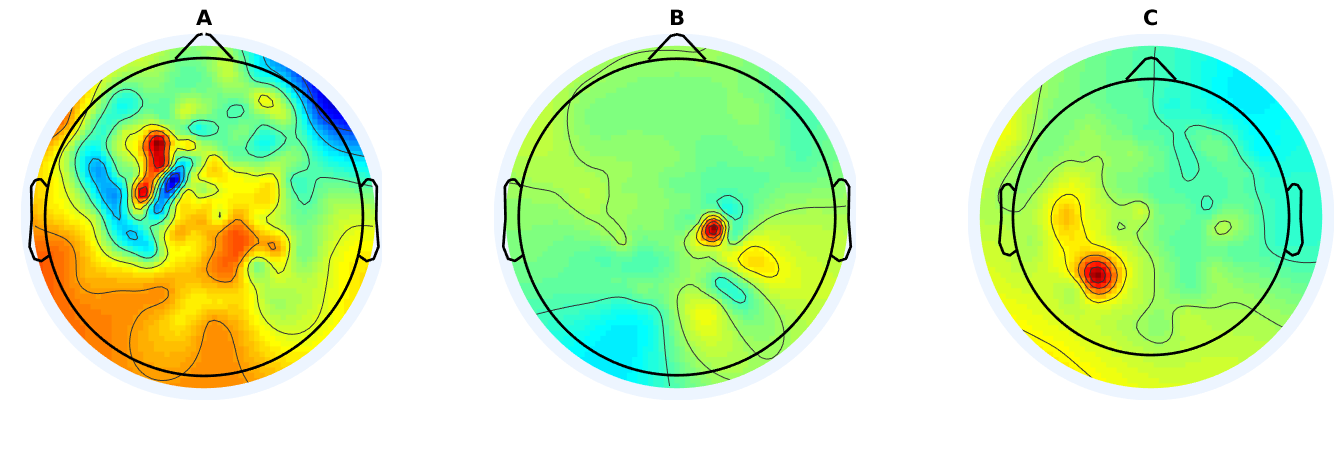
\includegraphics[width=\linewidth]{AllComponents.png}
  \caption{Graphical illustrations (using \cite{Delorme04eeglab}) of the independent components with features most correlated with audio features, from left to right, /{\em pah}/, /{\em pah tah kah}/ and verb generation experiments. These are generated using the ICA weight matrix interpolated over MEG sensor locations. Interestingly examples A and B}
  \label{fig:components}
\end{figure}
 
\subsubsection{All features vs. age}

When correlating with age, 172 features have significant values, all of which are MEG features. This includes the autocorrelation features of eight ICA components (including the first (highest entropy) component) in addition to the entire available frequency spectrum of four of these components. \hl{TODO: Re-visit these for what f-ranges they correspond to}.

The correlation of a single ICA component has correlation coefficients $\text{abs}(r)>0.3$ for nearly all of its features, which is true of no other components considered. \hl{TODO: image of this component} Three other components also have features with correlation $\text{abs}(r)>0.3$, for features that corresponded to various mean variants.

\message{ !name(frontiers.tex) !offset(408) }

\end{document}
